% Module dependencies of stdlib_Integrate, from the `use` statements of
% src/**/*.f90 (modules stdlib_integrate_<name>; the folder under each name): an arrow goes from a module to a module it uses, so everything
% points down. Only the arrows no other path implies are drawn (the transitive
% reduction): rk_steps also uses status directly, but depends on it
% through rk_generic anyway. stdlib_kinds (wp), used by nearly every
% module, is left out. Every module is hand-written.
\documentclass[tikz,border=6pt]{standalone}
\usetikzlibrary{arrows.meta,positioning,fit,backgrounds}

% Palette: modules grey, the umbrella module blue, groups light grey.
\definecolor{handcol}{RGB}{235,235,235}
\definecolor{topcol}{RGB}{214,230,245}
\definecolor{bandcol}{RGB}{247,247,247}

\begin{document}
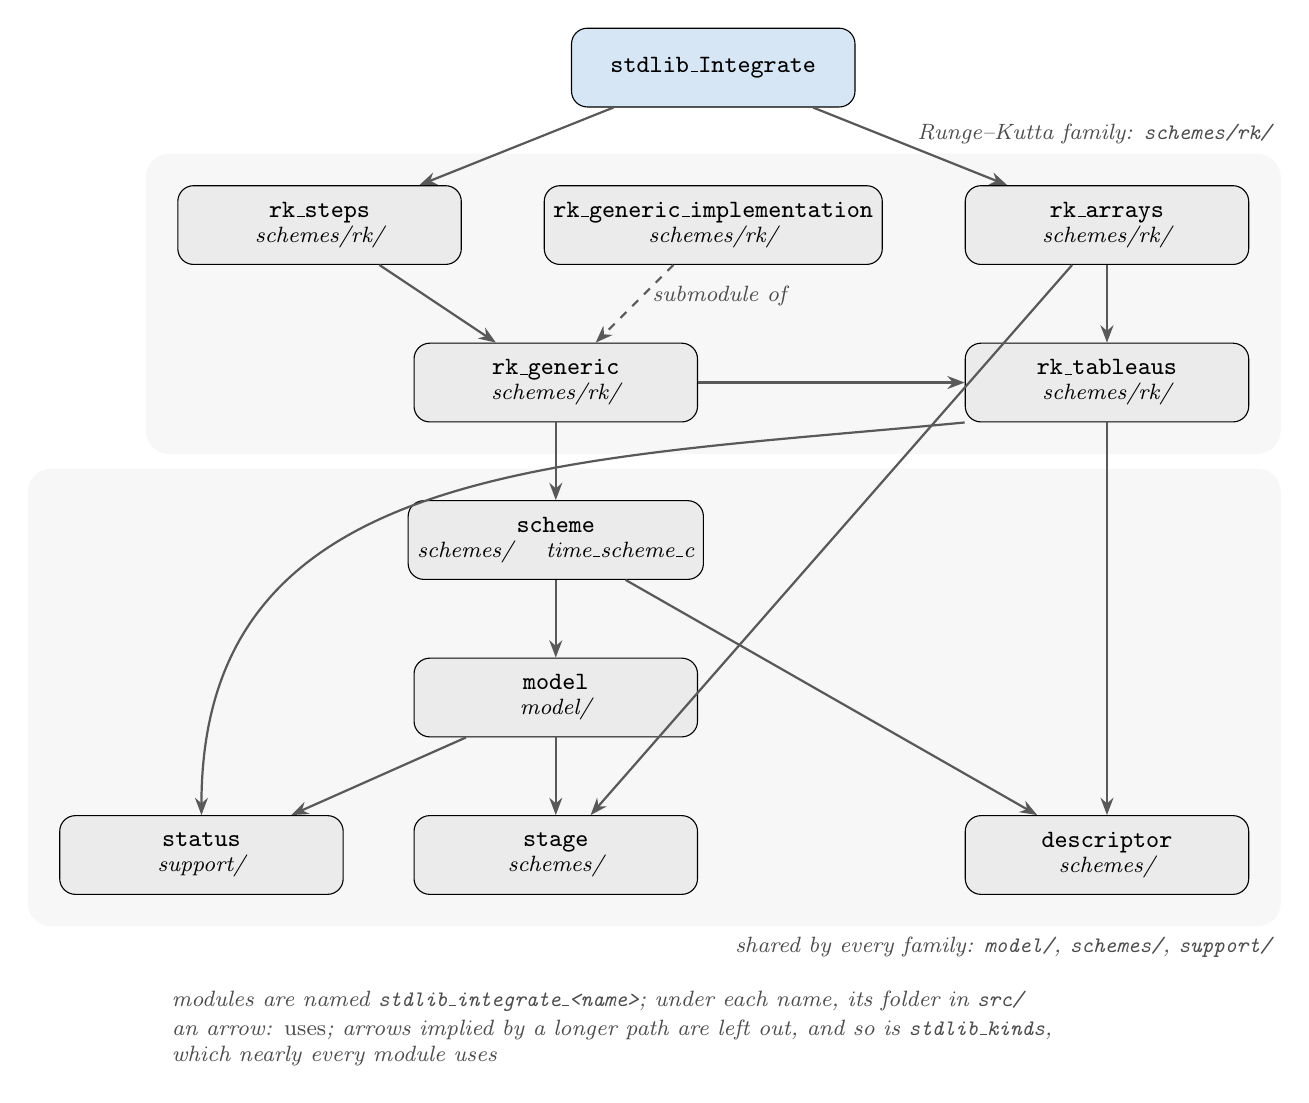
\begin{tikzpicture}[
    font=\small,
    >={Stealth[length=2.2mm]},
    mod/.style={draw, rounded corners=2mm, fill=handcol, minimum height=8mm,
                minimum width=36mm, minimum height=10mm, align=center, font=\small\ttfamily},    % a hand-written module
    ext/.style={mod, fill=white, dashed},                                  % an external dependency
    top/.style={mod, fill=topcol},                                         % the umbrella module
    uses/.style={->, thick, black!65},                                     % "uses"
    group/.style={fill=bandcol, rounded corners=3mm, inner sep=4mm},       % a group of modules
    grouplabel/.style={font=\footnotesize\itshape, text=black!70},         % its name
    note/.style={font=\footnotesize\itshape, text=black!70, align=left},   % explanatory note
  ]

  % ---- the umbrella ----
  \node[top] (umbrella) at (8, 12)   {stdlib\_Integrate};

  % ---- Runge-Kutta family ----
  \node[mod] (methods)  at (3, 10)   {rk\_steps\\[-2pt]{\footnotesize\rmfamily\itshape schemes/rk/}};
  \node[mod] (arrays)   at (13, 10)  {rk\_arrays\\[-2pt]{\footnotesize\rmfamily\itshape schemes/rk/}};
  \node[mod] (impl)     at (8, 10)   {rk\_generic\_implementation\\[-2pt]{\footnotesize\rmfamily\itshape schemes/rk/}};
  \node[mod] (generic)  at (6, 8)    {rk\_generic\\[-2pt]{\footnotesize\rmfamily\itshape schemes/rk/}};
  \node[mod] (tableaus) at (13, 8)   {rk\_tableaus\\[-2pt]{\footnotesize\rmfamily\itshape schemes/rk/}};

  % ---- core: shared by any family ----
  \node[mod] (abstract) at (6, 6)    {scheme\\[-2pt]{\footnotesize\rmfamily\itshape schemes/ \quad time\_scheme\_c}};
  \node[mod] (model)    at (6, 4)    {model\\[-2pt]{\footnotesize\rmfamily\itshape model/}};
  \node[mod] (status)   at (1.5, 2)  {status\\[-2pt]{\footnotesize\rmfamily\itshape support/}};
  \node[mod] (stage)    at (6, 2)    {stage\\[-2pt]{\footnotesize\rmfamily\itshape schemes/}};
  \node[mod] (method)   at (13, 2)   {descriptor\\[-2pt]{\footnotesize\rmfamily\itshape schemes/}};

  % ---- uses (transitive reduction) ----
  \draw[uses] (umbrella) -- (methods);
  \draw[uses] (umbrella) -- (arrays);
  \draw[uses] (methods)  -- (generic);
  \draw[uses, dashed] (impl) -- node[right, note, pos=0.4] {submodule of} (generic);
  \draw[uses] (generic)  -- (abstract);
  \draw[uses] (generic)  -- (tableaus);
  \draw[uses] (arrays)   -- (tableaus);
  \draw[uses] (arrays)   -- (stage);
  \draw[uses] (tableaus) -- (method);
  \draw[uses] (tableaus.south west) .. controls (6, 7) and (1.5, 7) .. (status.north);
  \draw[uses] (abstract) -- (model);
  \draw[uses] (abstract) -- (method);
  \draw[uses] (model)    -- (status);
  \draw[uses] (model)    -- (stage);

  % ---- groups, behind ----
  \begin{scope}[on background layer]
    \node[group, fit=(methods)(arrays)(impl)(generic)(tableaus),
          label={[grouplabel, anchor=south east]north east:Runge--Kutta family: \texttt{schemes/rk/}}] {};
    \node[group, fit=(abstract)(status)(method),
          label={[grouplabel, anchor=north east]south east:shared by every family: \texttt{model/}, \texttt{schemes/}, \texttt{support/}}] {};
  \end{scope}

  % ---- legend ----
  \node[note, anchor=north west] at (1.0, 0.4)
       {modules are named \texttt{stdlib\_integrate\_<name>}; under each name, its folder in \texttt{src/}\\[1pt]
        an arrow: \emph{uses}; arrows implied by a longer path are left out, and so is
        \texttt{stdlib\_kinds},\\ which nearly every module uses};
\end{tikzpicture}
\end{document}
